\documentclass[10pt]{beamer}

\usetheme[progressbar=frametitle]{metropolis}
\usepackage{appendixnumberbeamer}

\usepackage{booktabs}
\usepackage[scale=2]{ccicons}

\usepackage{pgfplots}
\usepgfplotslibrary{dateplot}

\usepackage{xspace}
\newcommand{\themename}{\textbf{\textsc{metropolis}}\xspace}

% \usepackage{graphicx}
% \usepackage{subcaption}

\title{UoE Maths Linux Server}
\subtitle{fORum Workshop}
% \date{\today}
\date{}
\author{Claire Zhang}
\institute{University of Edinburgh}
% \titlegraphic{\hfill
\includegraphics[height=0.8cm]{images/logo.png}}

\begin{document}

\maketitle

\begin{frame}{Table of contents}
  \setbeamertemplate{section in toc}[sections numbered]
  \tableofcontents%[hideallsubsections]
\end{frame}

\section[Intro]{Introduction}

\begin{frame}[fragile]{Maths Compute Servers}

Servers available\footnotemark:

\begin{itemize}
    \item \textbf{compute64x, compute64y and compute64z: }
    \begin{itemize}\scriptsize{
        \item {Dell PowerEdge R740 running Scientific Linux 7}
        \item 4 x Intel Gold 6234 3.3G, 8C/16T, 10.4GT/s, 24.75M Cache, Turbo, HT (130W) DDR4-2933
        \item 1.5TB local (not backed up) disk space (/data)}
    \end{itemize}
    \item \textbf{compute64c: }
    \begin{itemize}\scriptsize{
        \item Dell PowerEdge R920 running Scientific Linux 7
        \item Four Intel Xeon E7-4830 v2 2.2GHz, 20M Cache, 7.2 GT/s QPI, Turbo (4x10Cores) 256 GB RAM
        \item 750 GB local (not backed up) disk space (/data)}
    \end{itemize}
    \item \textbf{compute64d: }
    \begin{itemize}\scriptsize{
        \item Dell PowerEdge R430 running Scientific Linux 7
        \item Four Intel Xeon E5-2680 v3 2.5GHz, 30M Cache, 9.6 GT/s QPI 192 GB RAM
        \item 1.7 TB local (not backed up) disk space (/data)}
    \end{itemize}
\end{itemize}

\footnotetext[1]{\tiny{https://intranet.maths.ed.ac.uk/it-support/high-performance-computing/maths-compute-servers}}

\end{frame}

\begin{frame}[fragile]{Restrictions}

\begin{itemize}
    \item maximum 10 CPU cores at any time
    \item only 1 compute server at any time
    \item do not use a very large amount of RAM or CPU time
    \item run no longer than a week or so
    \item reboot in the early morning on the 2nd Monday of each month
\end{itemize}

To ensure that, we can use htop(talk about it later). 

\end{frame}

\begin{frame}[fragile]{Software}

\begin{itemize}
    \item install anything that does not require root/admin access
    \item if need additional software, ask the IT team
    \item more information and licences on software services website\footnotemark
\end{itemize}

\footnotetext[2]{\tiny{https://intranet.maths.ed.ac.uk/it-support/software}}

\end{frame}

\section{Connect to the Server}

\subsection{Connect using ssh}

\begin{frame}[fragile]{Connect using ssh}

\begin{figure}[!ht]
\centering

\includegraphics[width = 0.9\textwidth]{images/maths_server_connect_steps.png}
\end{figure}

\begin{itemize}
    \item \textbf{Gateway Servers}: ssh1, ssh2, ssh3
    \item \textbf{Maths Compute Server}: compute64x, compute64y, compute64z, compute64c, compute64d
    \newline
    \item Use eduroam or VPN
\end{itemize}

\end{frame}

\begin{frame}[fragile]{Connect using ssh\footnotemark}

\begin{itemize}
    \item{
    On \textbf{Linux} or \textbf{Mac}: terminal or \textbf{Windows}: PowerShell
    \begin{itemize}
        \item Command: ssh UUN@hostname.maths.ed.ac.uk
        \item{
        e.g., \underline{ssh s1234567@ssh1.maths.ed.ac.uk} (gateway)
        
        \quad \quad \underline{ssh s1234567@compute64x.maths.ed.ac.uk} (Maths compute)
        }
        \item login with password
    \end{itemize}
    }
    \hfill
    \item{
    On \textbf{Windows}: PuTTY, MobaXterm (not recommended)
    \begin{itemize}
        \item port: 22
        \item host: hostname.maths.ed.ac.uk
        \item login with UUN and password
        \item use the same command as above to connect to Maths compute server
    \end{itemize}
    }
\end{itemize}

\footnotetext[3]{\tiny{https://intranet.maths.ed.ac.uk/it-support/remote-login/howto-ssh}}

\end{frame}

\begin{frame}[fragile]{Once connected}

\begin{itemize}
    \item your space is /home/UUN
    \item create a folder in \textbf{/data} for efficiency (not backed up)
    \newline
    \item{
    \textbf{Basic Linux Commands: }
    \begin{itemize}
        \item {cd: navigate files and folder
        
        \quad e.g., cd data/; cd /home/UUN; cd ..}
        \item {ls: list files and folders under the current directory
        
        \quad e.g., ls; ls /data}
        \item {cp: copy files or folders
        
        \quad e.g., cp -r /home/UUN/project /data/UUN/}
        \item {mv: move files or folders (also used as rename)
        
        \quad e.g., mv -r /home/UUN/project /data/UUN/}
        \item {mkdir: make a directory)
        
        \quad e.g., mkdir /data/UUN}
        \item {rm: remove files or folders)
        
        \quad e.g., rm /home/UUN/project/*; rm -rf /*}
    \end{itemize}
    }
\end{itemize}

\end{frame}

\subsection{Useful Command Line Tools}

\begin{frame}[fragile]{Useful command line tools - htop}

\textbf{htop\footnotemark}: keep track of how much resource you are using

\begin{figure}[!ht]
\centering
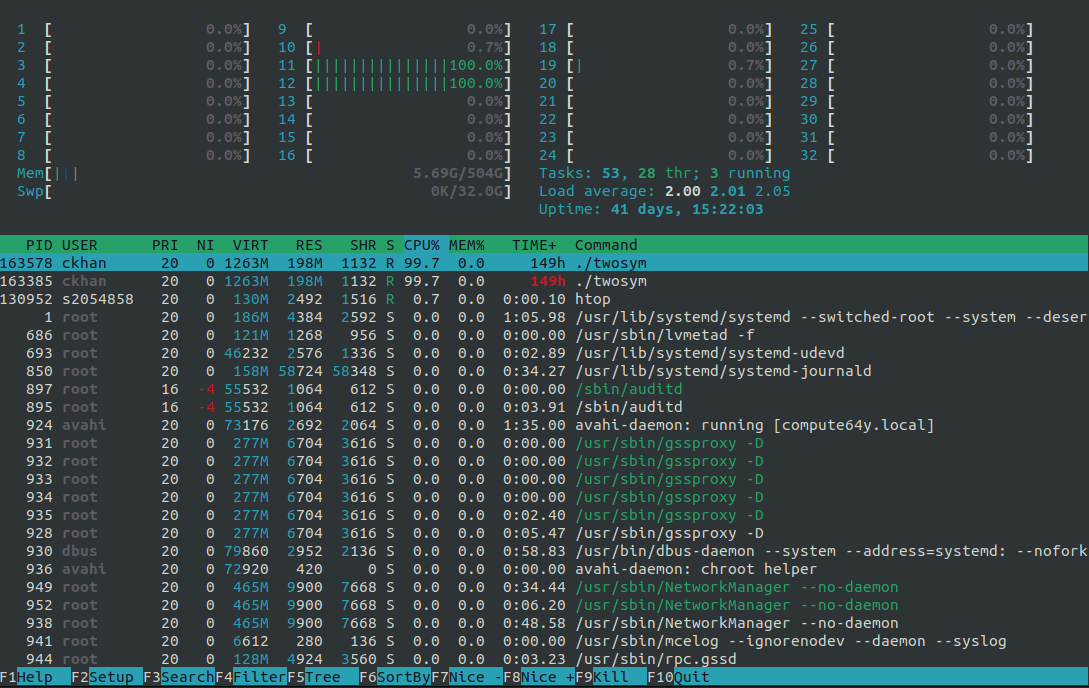
\includegraphics[width = 0.9\textwidth]{images/htop.png}
\end{figure}

\footnotetext[4]{\tiny{https://htop.dev/}}

\end{frame}

\begin{frame}[fragile]{Useful command line tools - tmux}

\textbf{tmux\footnotemark}: terminal multiplexer (split windows and detach)

\begin{figure}[!ht]
\centering
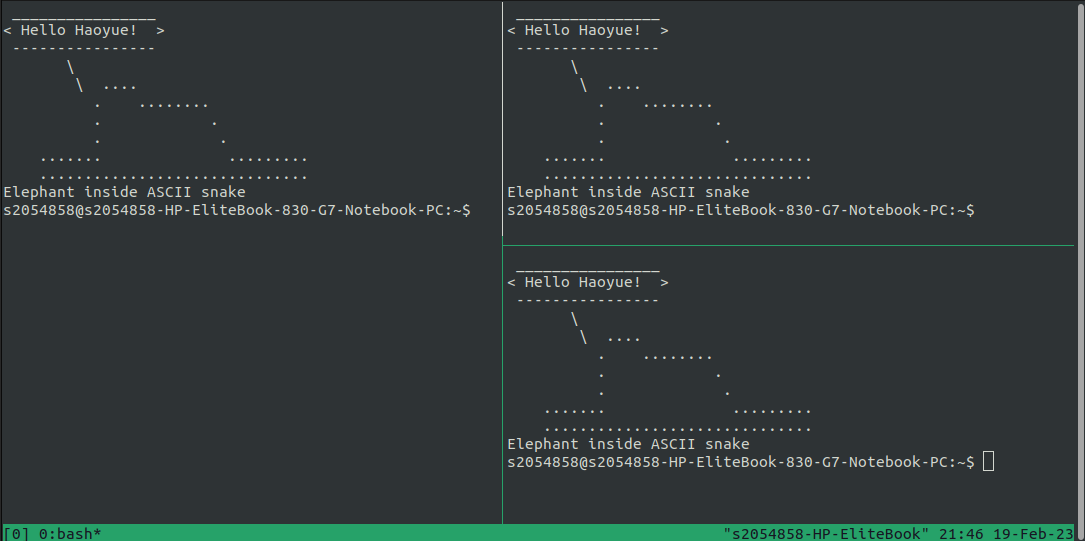
\includegraphics[width = 0.9\textwidth]{images/tmux.png}
\end{figure}

\footnotetext[5]{\tiny{https://github.com/tmux/tmux/wiki}}

\end{frame}

\begin{frame}[fragile]{Useful command line tools - tmux}

\textbf{tmux}: terminal multiplexer (split windows and detach)

\textbf{useful commands: }

\begin{itemize}
    \item in terminal: 
    {\begin{itemize}
        \item tmux new (or just tmux): create a new session
        \item tmux ls: list current sessions
        \item tmux attach: bring back the last detached session
        \item tmux attach -t <name>: bring back detached session named <name>
        \item tmux kill-session -t <name>: kill session named <name>
    \end{itemize}}
    \item in tmux sessions: 
    {\begin{itemize}
        \item ctrl D: exit
        \item ctrl B + \%: vertical split
        \item ctrl B + ": horizontal split
        \item ctrl B + D: detach (it will still run in the background)
    \end{itemize}}
\end{itemize}

\end{frame}

\begin{frame}[fragile]{Useful command line tools - X11}

\textbf{X11\footnotemark}: use GUI (a bit slow)

\begin{figure}[!ht]
\centering
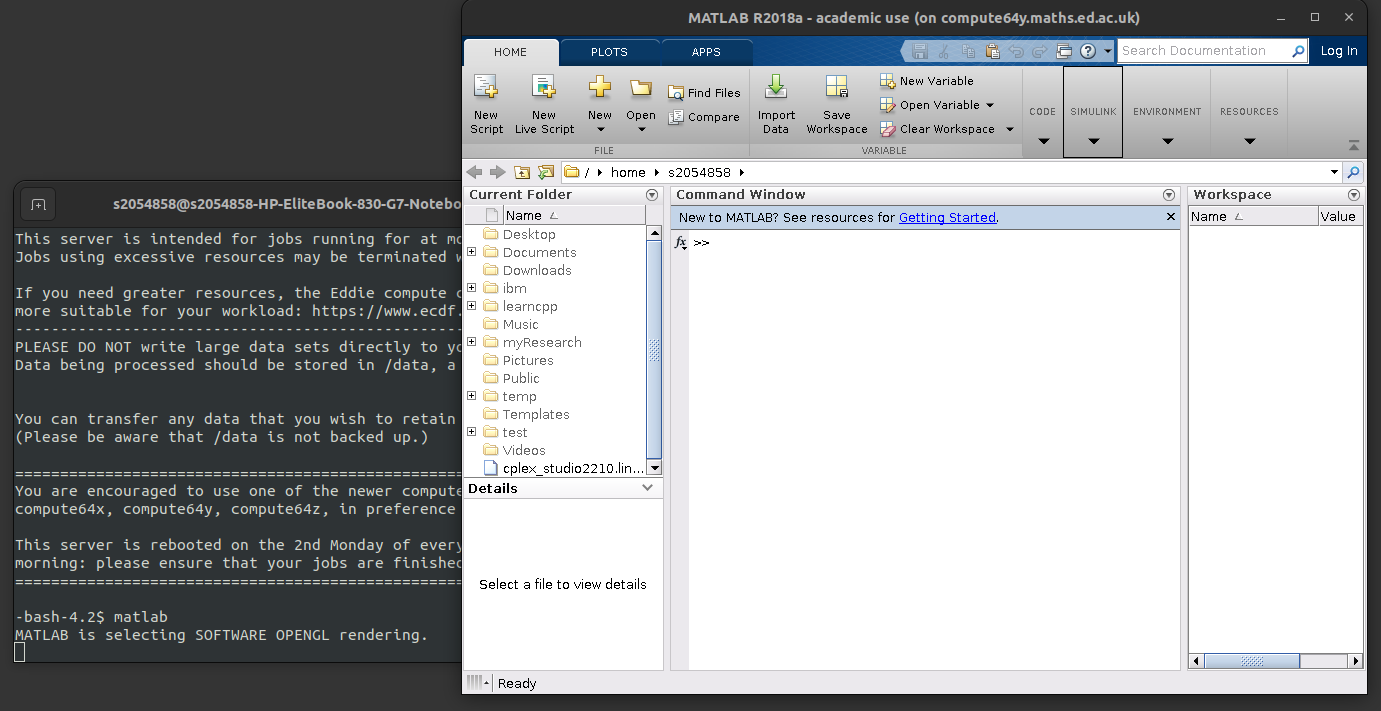
\includegraphics[width = 0.9\textwidth]{images/X11.png}
\end{figure}

\textbf{command}: ssh \textbf{-X} UUN@hostname.maths.ed.ac.uk

\hfill

\footnotetext[6]{\tiny{https://www.x.org/wiki/Releases/7.7/}}

\end{frame}

\begin{frame}[fragile]{Useful command line tools - text editor}

\textbf{vi, vim\footnotemark, nano\footnotemark... }

\begin{figure}[!ht]
\centering
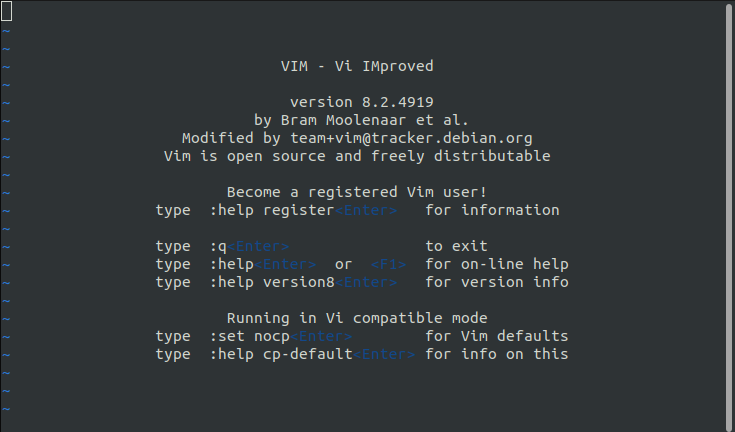
\includegraphics[width = 0.8\textwidth]{images/vi.png}
\end{figure}

\footnotetext[7]{\tiny{https://github.com/vim/vim}}
\footnotetext[8]{\tiny{https://www.nano-editor.org/}}

\end{frame}

\begin{frame}[fragile]{Useful command line tools - text editor}

\textbf{vi, vim, nano... }

\begin{figure}[!ht]
\centering

\includegraphics[width = 0.6\textwidth]{images/vim_meme.jpg}
\end{figure}

\scriptsize{\textbf{More information on how to exit vim}: https://github.com/hakluke/how-to-exit-vim}

\end{frame}

\begin{frame}[fragile]{Useful command line tools - scp}

\textbf{scp}: (securely copy) transfer files remotely

\hfill

\textbf{command}: 
\begin{itemize}
    \item {server -> local: 
    
    scp username@from\_host:directory /local\_directory}
    \item {local -> server: 
    
    scp /local\_directory username@from\_host:directory}
\end{itemize}

\quad e.g., scp -r s1234567@ssh1.maths.ed.ac.uk:/home/s1234567/project /home/my\_projects/

\end{frame}

\subsection{Connect using Remote Desktop}

\begin{frame}[fragile]{Connect using Remote Desktop\footnotemark}

graphical Linux desktop environment

\begin{figure}[!ht]
\centering
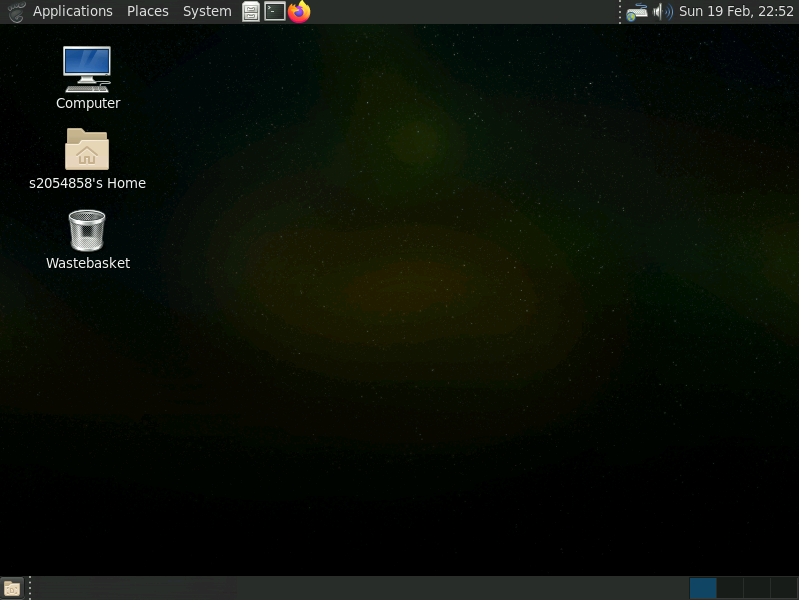
\includegraphics[width = 0.7\textwidth]{images/Remote_Desktop.png}
\end{figure}

\footnotetext[9]{\tiny{https://intranet.maths.ed.ac.uk/it-support/remote-login/linux-remote-desktop}}

\end{frame}

\begin{frame}[fragile]{When to use? }

For efficiency reasons, it is not recommended to use the graphic environment. 

Use the remote desktop if you only need access to your file but not the software.

\textbf{Recommended software}: 

\begin{itemize}
    \item \textbf{Windows}: Remote Desktop client program
    \item \textbf{Mac}: Microsoft Remote Desktop 10
    \item \textbf{Linux}: Vinagre and Remmina
\end{itemize}

\hfill

\scriptsize{\textbf{More information on}: https://intranet.maths.ed.ac.uk/it-support/remote-login/linux-remote-desktop}

\end{frame}

\end{document}
